\subsubsection{Caso d'uso UC8.1.3.1: Creazione domanda vero/falso}
	\label{UC8.1.3.1}
	\begin{figure}[h]
		\centering
			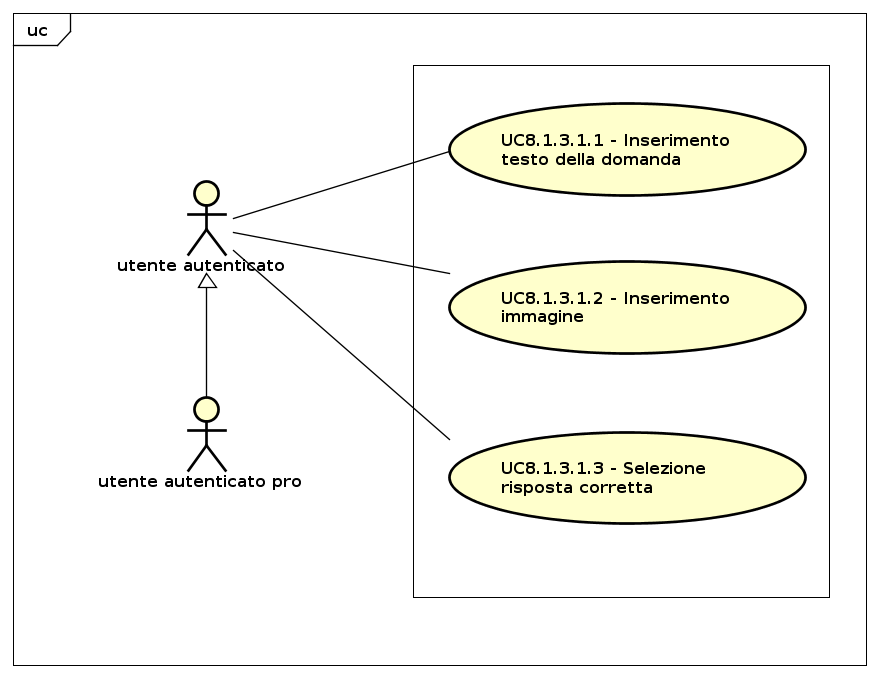
\includegraphics[scale=0.45,keepaspectratio]{UML/UC8_1_3_1.png}
		\caption{UC8.1.3.1: Creazione domanda vero/falso}
	\end{figure}
	\FloatBarrier
	\begin{itemize}
		\item
			\textbf{Attori}: utente autenticato, utente autenticato pro;
		\item		
			\textbf{Descrizione}: lo scopo di questa funzionalità è offrire agli attori la possibilità di creare domande vero/falso;
		\item
			\textbf{Precondizione}: gli attori hanno selezionato la seguente funzionalità; 
		\item
			\textbf{Postcondizione}: gli attori hanno creato una domanda vero/falso;
		\item
			\textbf{Scenario principale}:
	       		\begin{enumerate}
	       			\item
	       			Gli attori devono compilare il campo dati destinato alla scrittura del testo della domanda (UC8.1.3.1.1)
	       			\item
	       			Gli attori possono inserire un'immagine relativa al testo della domanda (UC8.1.3.1.2)
					\item
					Gli attori devono indicare la risposta corretta tramite uno strumento di selezione (UC8.1.3.1.3).
	 			\end{enumerate}
	\end{itemize}

\subsubsection{Caso d'uso UC8.1.3.1.1: Inserimento testo della domanda}
	\begin{itemize}
		\item
			\textbf{Attori}: utente autenticato, utente autenticato pro;
		\item		
			\textbf{Descrizione}: lo scopo di questa funzionalità è offrire agli attori la possibilità di inserire il testo della domanda;
		\item
			\textbf{Precondizione}: gli attori hanno selezionato la modalità di creazione di una domanda vero/falso; 
		\item
			\textbf{Postcondizione}: gli attori hanno inserito il testo della domanda;
		\item
			\textbf{Scenario principale}: gli attori inseriscono il testo della domanda. 
	 			
	\end{itemize}
	
\subsubsection{Caso d'uso UC8.1.3.1.2: Inserimento immagine}
	\begin{itemize}
		\item
			\textbf{Attori}: utente autenticato, utente autenticato pro;
		\item		
			\textbf{Descrizione}: lo scopo di questa funzionalità è offrire agli attori la possibilità di inserire un'immagine relativa al testo della domanda;
		\item
			\textbf{Precondizione}: gli attori hanno selezionato la modalità di creazione di una domanda vero/falso; 
		\item
			\textbf{Postcondizione}: gli attori hanno inserito l'immagine;
		\item
			\textbf{Scenario principale}: gli attori inseriscono l'immagine. 	
	\end{itemize}
	

\subsubsection{Caso d'uso UC8.1.3.1.3: Selezione risposta corretta}
	\begin{itemize}
		\item
			\textbf{Attori}: utente autenticato, utente autenticato pro;
		\item		
			\textbf{Descrizione}: lo scopo di questa funzionalità è offrire agli attori la possibilità, tramite uno strumento di selezione, di indicare la risposta corretta;
		\item
			\textbf{Precondizione}: gli attori hanno selezionato la modalità di creazione di una domanda vero/falso; 
		\item
			\textbf{Postcondizione}: gli attori hanno selezionato la risposta corretta;
		\item
			\textbf{Scenario principale}: gli attori indicano la risposta corretta tramite uno strumento di selezione. 
	 			
	\end{itemize}
	

	
